%\documentclass[12pt,draft]{article}
\documentclass[12pt,draft]{article}
\usepackage{amsmath}
\usepackage{amsfonts}
\usepackage{times}
\usepackage{graphicx}
\usepackage{color}
\usepackage{multirow}
%
\usepackage[authoryear]{natbib}
%
\usepackage{rotating}
\usepackage{bbm}
\usepackage{latexsym}
%\DeclareGraphicsExtensions{.eps,.png}

% reference links
\usepackage{nameref,hyperref}
\usepackage[table]{xcolor}
\hypersetup{
	colorlinks = true,                    % text and not border
	citecolor = {teal},
	linkcolor = {purple},
}
% black, blue, brown, cyan, darkgray, gray, green, lightgray, lime, 
% magenta, olive, orange, pink, purple, red, teal, violet, white, yellow.

%%% margins 
\textheight 23.4cm
\textwidth 14.65cm
\oddsidemargin 0.375in
\evensidemargin 0.375in
\topmargin  -0.55in
%
%\renewcommand{\baselinestretch}{2}
%
\interfootnotelinepenalty=10000
%
\renewcommand{\thesubsubsection}{\arabic{section}.\arabic{subsubsection}}
\newcommand{\myparagraph}[1]{\ \\{\em #1}.\ \ }
\newcommand{\citealtt}[1]{\citeauthor{#1},\citeyear{#1}}
\newcommand{\myycite}[1]{\citep{#1}}

% Different font in captions
\newcommand{\captionfonts}{\normalsize}

\makeatletter  
\long\def\@makecaption#1#2{%
	\vskip\abovecaptionskip
	\sbox\@tempboxa{{\captionfonts #1: #2}}%
	\ifdim \wd\@tempboxa >\hsize
	{\captionfonts #1: #2\par}
	\else
	\hbox to\hsize{\hfil\box\@tempboxa\hfil}%
	\fi
	\vskip\belowcaptionskip}
\makeatother   
%%%%%

\renewcommand{\thefootnote}{\normalsize \arabic{footnote}} 	

\newcommand\norm[1]{\left\lVert#1\right\rVert}

\usepackage{mathtools}
\newcommand{\defeq}{\vcentcolon=}

\newcommand{\fullderiv}[2]{\frac{\mathrm{d}#1}{\mathrm{d}#2}}
\newcommand{\partderiv}[2]{\frac{\partial#1}{\partial#2}}
\newcommand{\avg}[2]{\left\langle #1\right\rangle_{#2}}


\begin{document}
	\hspace{13.9cm}1
	
	\ \vspace{20mm}\\
	
	{\LARGE\noindent Optimizing individually the variance of the
		neural activity regulates the echo-state spectral radius}
	
	\ \\
	{\bf \large Fabian Schubert and Claudius Gros}\\
	{Institute for Theoretical Physics, Goethe University, Frankfurt a.M., Germany.}\\
	%
	
	%\ \\[-2mm]
	\noindent
	{\bf Keywords:} variance optimization, echo state network, spectral radius, 
	biological plausibility, self-organization, universality
	
	\thispagestyle{empty}
	\markboth{}{Variance optimization}
	%
	\ \vspace{-0mm}\\
	
	\section{Introduction}
	\the\textwidth
	
	Strategies for the optimization of ESN hyperparameters can be divided in two categories: supervised and unsupervised methods, where the first one utilizes an error signal, while the latter only uses information contained within the network dynamics.
	
	In the first part of our research, we investigated the possibility of defining an unsupervised homeostatic mechanism that controls the mean and variance of neuronal firing in such a way that the network acts in a regime that yields good performance in sequence learning tasks. This mechanism acts on two sets of parameters, biases $b_i$ and neural gain factors $a_i$. It should be emphasized that we did not attempt to define an arbitrarily complex measure that would be most suitable for optimization, e.g. from a machine learning perspective. Rather, we restricted ourselves to adhere to �biologically plausible' mechanisms. While no exact definition of this term exists, it embraced two aspects in our work:
	\begin{itemize}
		\item The dynamics of all variables must be local, i.e., they are bound to a specific neuron and may only access other variables that are locally accessible. In a strict sense, this consists of all other dynamic variables of the neuron itself and information about the activity of adjacent neurons. Being less restrictive, one could claim that it should also be possible to access aggregate or �mean-field' quantities, that average a property over the entire population.
		\item We use a time-discrete model where the state of a variable in the next step may only be determined by states of the previous step. This means that information about past states must be integrated dynamically.
	\end{itemize} 
	
	 Our approach was based on the assumption that network performance is optimal when the spectral radius of the effective recurrent connectivity, given by $a_i W_{ij}$, is close to, but slightly below $1$. We attempted to transfer this non-local measure into a condition that could be implemented in a biologically plausible way. 
	
	\section{Model}
	\subsection{Network dynamics}
	\begin{align}
		y_i(t) &= \tanh\left(x_i(t) - b_i\right) \\
		x_i(t) &= X_{{\rm r},i}(t) + X_{{\rm e},i}(t) \\
		X_{{\rm r},i}(t) &= a_i \sum_{j=1}^N W_{ij} y_j(t-1) \\
		X_{{\rm e},i}(t) &= \sum_{j=1}^{D_{\rm in}} W^{\rm u}_{ij} u_j(t) \\
		o_i(t) &= o^0_i + \sum_{j=1}^{D_{\rm out}} W^{\rm o}_{ij} y_j(t)
	\end{align}
	where $\mathbf{y}, \mathbf{x}, \mathbf{a}, \mathbf{b}  \in \mathbb{R}^N$, $W \in \mathbb{R}^{N \times N}$, $\mathbf{u} \in \mathbb{R}^{D_{\rm in}}$, $W^{\rm u} \in \mathbb{R}^{N \times D_{\rm in}}$, $\mathbf{o}, \mathbf{o}^0 \in \mathbb{R}^{D_{\rm out}}$ and  $W^{\rm o} \in \mathbb{R}^{D_{\rm out} \times N}$.
	
	Furthermore
	\begin{align}
		\mathrm{p}\left(W_{ij} = x\right) &= \begin{cases}
		\delta(x) & i=j \\
		p_{\rm r} \mathcal{N}\left(x,\mu=0,\sigma=\sigma_{\rm w}/\sqrt{Np_{\rm r}} \right) + (1-p_{\rm r}) \delta(x) & \mathrm{else}
		\end{cases} \\
		\mathrm{p}\left(W^{\rm u}_{ij} = x\right) &= \mathcal{N}\left(x,\mu=0,\sigma=1\right) \; .
	\end{align}
	
	Initially, we chose $N=1000$ as the network size, however, due to computational complexity, the results presented here are generated with a network of size $N=500$, unless stated otherwise. See Table~\ref{tab:net_params} for the standard network parameters.
	\begin{table}
		\centering
		\renewcommand{\arraystretch}{1.2}
		\caption{Standard network parameters.}
		\begin{tabular}{c|c|c|c|c}
			$N$ & $D_{\rm in}$ & $D_{\rm out}$ & $p_{\rm r}$ & $\sigma_{\rm w}$ \\ \hline
			500 & 1 & 1 & 0.1 & 1
		\end{tabular}
		\label{tab:net_params}
	\end{table}
	\subsection{Homeostatic Adaptation}
	For our homeostatic update mechanism, we use the following dynamics:
	\begin{align}
		b_i(t) &= b_i(t-1) + \epsilon_{\rm b} \left[y_i(t) - \mu^{\rm t}_i \right] \\
		\mu^{\rm y}_i(t) &= \left[1 - \epsilon_{\mu}\right] \mu^{\rm y}_i(t-1) + \epsilon_{\mu} y_i(t) \\
		a_i(t) &= a_i(t-1) + \epsilon_{\rm a} [{\sigma^{\rm t}_i}^2 - \left( y_i(t) - \mu^{\rm y}_i(t) \right)^2] \; .
	\end{align}
	See Table~\ref{tab:hom_params} for the standard values.
	
	\begin{table}
		\centering
		\renewcommand{\arraystretch}{1.2}
		\caption{Standard homeostasis parameters.}
		\begin{tabular}{c|c|c|c|c}
			$\epsilon_{\rm b}$ & $\epsilon_{\mu}$ & $\epsilon_{\rm a}$ & $\mu^{\rm t}_i$ & $\sigma^{\rm t}_i$\\ \hline
			$10^{-3}$ & $10^{-4}$ & $10^{-3}$ & $0.05$ & variable 
		\end{tabular}
		\label{tab:hom_params}
	\end{table}

\section{Theory}
We stated in the model description that all recurrent weights were drawn independently from a sparse Gaussian distribution. In some sense, of course, this is an assumption that already fulfills one of the conditions that is known to make ESNs work, namely a balance between excitation and inhibition. However, since adjusting gains does not provide a means to dynamically achieve this property, we had to take it as given.

Furthermore, we assumed that all entries of the weight matrix were independently drawn from the same distribution. Under this assumption, using the circular law, it follows that setting all gain values to $1/\sigma_{\rm w}$ will result in a uniform unit circle distribution of eigenvalues. The situation is less clear if we allow the rows or columns of the matrix to follow different distributions, in particular---since we assumed to have zero mean---different variances. Numerically, we found that if
\begin{equation}
R_{\rm a} \equiv \avg{R_{{\rm a},i}}{\rm P} = \avg{a^2_i \sum_j W_{ij}}{\rm P} = 1
\end{equation}
where $\sigma^2_{{\rm w},i}$ are the variances of individual rows of the matrix, the spectral radius will be unity. This observation was also reported and proven in \citep{Rajan2006}.

From this observation, two question emerge: first, can we find local gain dynamics that can tune the global measure $R_{\rm a}$? And second, given the assumption that this constraint is fulfilled, does the particular distribution of gains affect the network performance?

Since $R_{\rm a}$ is already a population average itself, we could simply argue that a biologically plausible mechanism that adjusts gains proportionally would be
\begin{equation}
a_i(t+1) = a_i(t) + \epsilon_{\rm a} a_i(t) \left[R^t_{\rm a} - R_{\rm a}(t) \right]
\end{equation}
where $R^t_{\rm a}$ is the spectral radius we would like to achieve.

The question at hand is: could a diffusive neuromodulator encode the squared product of the neural gain and the variance of its synaptic weights? Or, alternatively, could this quantity be encoded in a different physical variable?

\subsection{Spectral Radius Encoded in Input and Neural Activity}

One possible way to encode the aforementioned quantity in physical way is based on the very general statement that each configuration of gains, weights and input statistics will yield a particular set of statistics for the resulting neural activity. Therefore, we hypothesized that it should be possible to establish an (approximate) description of the causal relation of these properties. In particular, this would potentially allow us to link a given value of $R_{\rm a}$, expressed as a function of gains and weights, to a corresponding set of input and neural activity statistics.

Based on this approach, we came up with an approximate self-consistency equation that was based on the following assumptions/simplifications:

\begin{itemize}
	\item We reduced the set of gains $a_i$ to single variable $a$.
	\item Every neuron receives statistically independent external input, which is however drawn from the same statistic characterized by the standard deviation $\sigma_{\rm ext}$. We assumed the mean input to be zero.
	\item Each neurons has the same homeostatic target variance.
	\item We ignore cross-correlations of activity in the neural population. Furthermore, we also assumed that each neuron has zero autocorrelation for $\tau \neq 0$.
	\item Even though the external input signal could in theory follow an arbitrary statistical distribution, we model the statistics of the sum of recurrent and external input with a Gaussian distribution.
	\item We ignore the small offset $\mu^{\rm t}_i$ in the mean activity.
\end{itemize}

Under these assumptions, the networks fulfills a self-consistency equation given by

\begin{equation}
\sigma_{\rm t}^2=\int_{-\infty}^{\infty}
{\rm dx}\tanh^2(x) N_{\mu,\sigma}(x),
\qquad \mu = 0, \quad
\sigma^2=a^2 \sigma_{\rm w}^2\sigma_{\rm t}^2+\sigma_{\rm ext}^2\,,
\label{self_consistency_x}
\end{equation}
%
where the distribution $N_{\mu,\sigma}(x)$ is 
of the membrane potential $x$ is a Gaussian, with mean $\mu=0$
and variance $\sigma^2$.
%A variable transformation $ax=z$ leads to
%%
%\begin{equation}
%\sigma_{\rm t}^2=\int_{-\infty}^{\infty}
%{\rm dz}\tanh^2(z) \frac{1}{\sqrt{2\pi\sigma_{\rm a}^2}}
%\mathrm{e}^{-z^2/2\sigma_{\rm a}^2}
%\qquad\quad
%\sigma_{\rm a}^2=a^2\big(\sigma_{\rm w}^2\sigma_{\rm t}^2+\sigma_{\rm ext}^2\big)\,,
%\label{self_consistency_z}
%\end{equation}
%%
%where the renormalized variance $\sigma_{\rm a}^2$ can
%be written as
%%
%\begin{equation}
%\sigma_{\rm a}^2=
%a^2\sigma_{\rm w}^2\big(\sigma_{\rm t}^2+\sigma_{\rm ext}^2/\sigma_{\rm w}^2\big)\,.
%\label{sigma_a_renormalized}
%\end{equation}
%
The gain $a$ is adapted such that \eqref{self_consistency_x}
is fulfilled, defining a 2d-manifold in the $(\sigma_{\rm t},\sigma_{\rm ext},a)$ space.

As a `sanity check', we ran a network simulation where the second and fourth approximation was actually exact. That is, we used Gaussian white noise with zero mean and $\sigma_{\rm ext}$	standard deviation for all neurons. Furthermore, the target mean was set to zero. Running the network for different pairs of external input variance and target variance, we got the results shown in Fig.~\ref{fig:gains_self_consist_hom_gauss}. The theoretical prediction given by \eqref{self_consistency_x} provides a good estimate for the population average of the squared gains.

\begin{figure}
	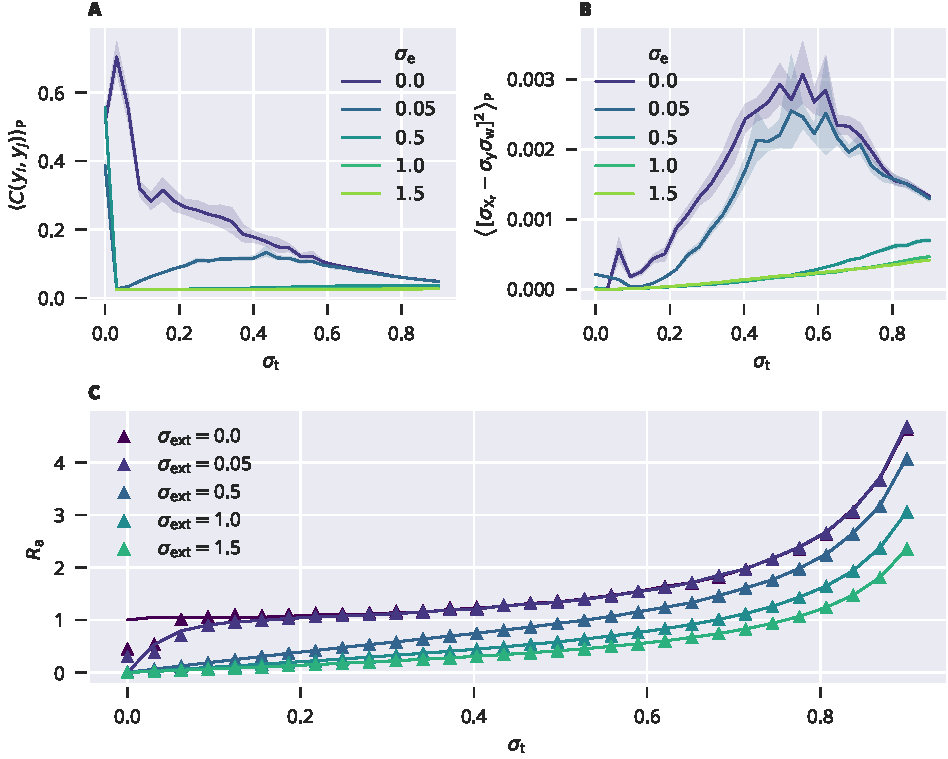
\includegraphics{./plots/homogeneous_independent_gaussian_input_compos.pdf}
	\caption{Homogeneous Independent Gaussian Input. {\bf A}: Population average of inter-neuron cross correlation. {\bf B}: Prediction error of recurrent input variance. {\bf C}: Theoretical prediction of $R_{\rm a}$ vs. numerical results.}
	\label{fig:gains_self_consist_hom_gauss}
\end{figure}

After this, we relaxed the assumptions and tested combinations of three variants: first, by introducing a variation in input variances by drawing input weights from a normal distribution whose variance was given by $\sigma_{\rm ext}^2$, see Fig.~\ref{fig:gains_self_consist_het_gauss}. Second, instead of independent Gaussian driving, we fed an identical binary input into every node, but input weights were the same, see Fig.~\ref{fig:gains_self_consist_hom_bin}. Third, we tested a combination of both previous variants, see Fig.~\ref{fig:gains_self_consist_het_bin}.

Comparing the results of these simulations, we can generally state that the quality of the gain depends on the amount of error within the prediction of the recurrent membrane variance: while errors are quite low in the autonomous case, they can be significantly increased (Fig.~\ref{fig:gains_self_consist_hom_bin} and \ref{fig:gains_self_consist_het_bin}) or further decreased (Fig.~\ref{fig:gains_self_consist_hom_gauss} and \ref{fig:gains_self_consist_het_gauss}), depending on the statistical properties of the external driving.



\begin{figure}
	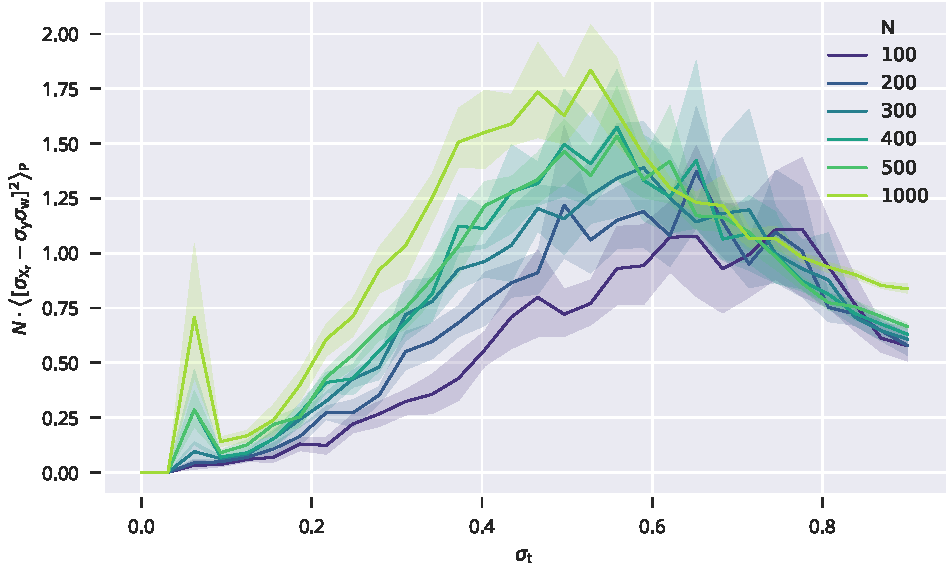
\includegraphics{./plots/homogeneous_independent_gaussian_input_rec_mem_pot_predict_size_scaling.pdf}
	\caption{Squared Recurrent Input Variance Prediction Error for homogeneous independent Gaussian input.}
	\label{fig:rec_var_prediction}
\end{figure}



In Echo state networks, the best task performance is usually found for a spectral radius close to unity. Therefore, our idea was to find an implicit expression for the spectral radius being one. As shown in Fig.~\ref{fig:gains_self_consist_hom_gauss}, \ref{fig:gains_self_consist_het_gauss}, \ref{fig:gains_self_consist_hom_bin} and \ref{fig:gains_self_consist_het_bin}, for a given external driving there exists a unique target activity variance that corresponds to a spectral radius of one.

Before proceeding to an analytical approach to this idea, we ran a numeric test by running a parameter sweep over pairs of $\sigma_{\rm t},\sigma_{\rm ext}$, adhering to the most simplified version, where each neuron received independent Gaussian external input with the same variance. The resulting transition line is shown in Fig.~\ref{Fig:theory_simulation_2}. Finding an analytic expression for this line would allow tuning the network into this transition point by measuring external and recurrent input variance. The following section explains an approximation method for finding an expression for this transition.
\subsection{Gaussian Approximation}
A polynomial approximation of $\tanh^2$ to fourth order captures the right behavior close to the origin, but does not account for the fact that $\tanh^2$ converges to $1$ for large absolute values of the membrane potential. Alternatively, an approximation with the correct scaling to second order as well as the right convergence is
\begin{equation}
\tanh^2(x) \approx 1 - \exp\left(-x^2 \right) \; .
\end{equation}
Using this approximation in \eqref{self_consistency_x} and solving the integral yields
\begin{equation}
\sigma^2_{\rm t} = 1 - 1/\sqrt{1+2a^2\sigma^2_{\rm w} \sigma^2_{\rm t} + 2\sigma^2_{\rm ext} } \; . \label{eq:gaussian_approx}
\end{equation}
Solving this equation for $a$ gives
\begin{equation}
a = \sigma_{\rm w}^{-1} \sqrt{\frac{1-\left(1-\sigma_{\rm t}^2\right)^2\left(1+2\sigma^2_{\rm ext}\right)}{2\left(1-\sigma^2_{\rm t}\right)^2\sigma^2_{\rm t}}} \; . \label{eq:gain_gaussian_approx}
\end{equation}

We can also derive an approximation for the critical transition from \eqref{eq:gaussian_approx}, which is given by
\begin{equation}
\sigma_{\rm ext} = \sqrt{\frac{1}{2\left(1-\sigma^2_{\rm t}\right)^2} -\sigma^2_{\rm t} - \frac{1}{2}} \; . \label{eq:crit_transition_gaussian_approx}
\end{equation} 
See Fig.~\ref{Fig:theory_simulation_2} for a comparison. One can obtain an even simpler approximation by
\begin{align}
\sigma_{\rm ext} &= \sqrt{\frac{1}{2\left(1-\sigma^2_{\rm t}\right)^2} -\sigma^2_{\rm t} - \frac{1}{2}} \label{eq:crit_transition_gaussian_approx_2} \\
&= \sqrt{2}^{-1}\sqrt{\frac{1}{\left(1-\sigma_{\rm t}^2\right)^2} - 2\sigma_{\rm t}^2 - 1} \\
&= \sqrt{2}^{-1}\frac{\sqrt{3\sigma_{\rm t}^4-2\sigma_{\rm t}^6}}{1-\sigma_{\rm t}^2} \\
&\approx \sqrt{\frac{3}{2}}\frac{\sigma_{\rm t}^2}{1-\sigma_{\rm t}^2} \label{eq:gauss_approx_approx}
\end{align}
where we ignored the sixth order term. \eqref{eq:gauss_approx_approx} is also shown in Fig.~\ref{Fig:theory_simulation_2} for comparison. This simple form also allows us conveniently state the inverse relation, which is what is required for tuning the network activity into an optimal state:
\begin{equation}
\sigma_{\rm t} \approx 1/ \sqrt{\sqrt{\frac{3}{2}} \sigma^{-1}_{\rm ext} +1} \; .
\end{equation}

{\bf However, this result is only valid for the particular case described: independent homogeneous Gaussian input.} As Fig.~\ref{fig:gains_self_consist_het_gauss} -- \ref{fig:gains_self_consist_het_bin} indicate, the manifold of the set of solutions can significantly change its shape, depending on particular input statistics---heterogeneity in the external input variance apparently being the dominant factor. In principle, this heterogeneity could be accounted for by modifying \eqref{eq:gaussian_approx} to only represent a local per-node condition:
\begin{equation}
\sigma^2_{\rm t,i} = 1 - 1/\sqrt{1+2a_i^2\sigma^2_{\rm w,i} \left\langle \sigma^2_{\rm t,i} \right\rangle_{\rm P} + 2 \sigma^2_{\rm ext,i} } \; . \label{eq:gaussian_approx_local}
\end{equation}
Averaging over this yields a much more complex self-consistency equation:
\begin{equation}
\left\langle \sigma^2_{\rm t,i} \right\rangle_{\rm P} = 1 - \left\langle 1/\sqrt{1+2a_i^2\sigma^2_{\rm w,i} \left\langle \sigma^2_{\rm t,i} \right\rangle_{\rm P} + 2\sigma^2_{\rm ext,i}} \right\rangle_{\rm P}\; . \label{eq:gaussian_approx_local_2}
\end{equation}
In this more general case, the critical transition would be defined by $\left\langle a_i^2 \sigma^2_{\rm w,i} \right\rangle_{\rm P} = 1$. Apart from the difficulties of finding the set of possible variance solutions for this condition, it is evident that it would depend on information about all external input variances, violating the assumptions we made about biological plausibility, even if we restrict ourselves to the more uniform case of $a_i^2 \sigma^2_{\rm w,i} = 1, \; \forall i$.

\begin{figure}[t!]
	\begin{center}
		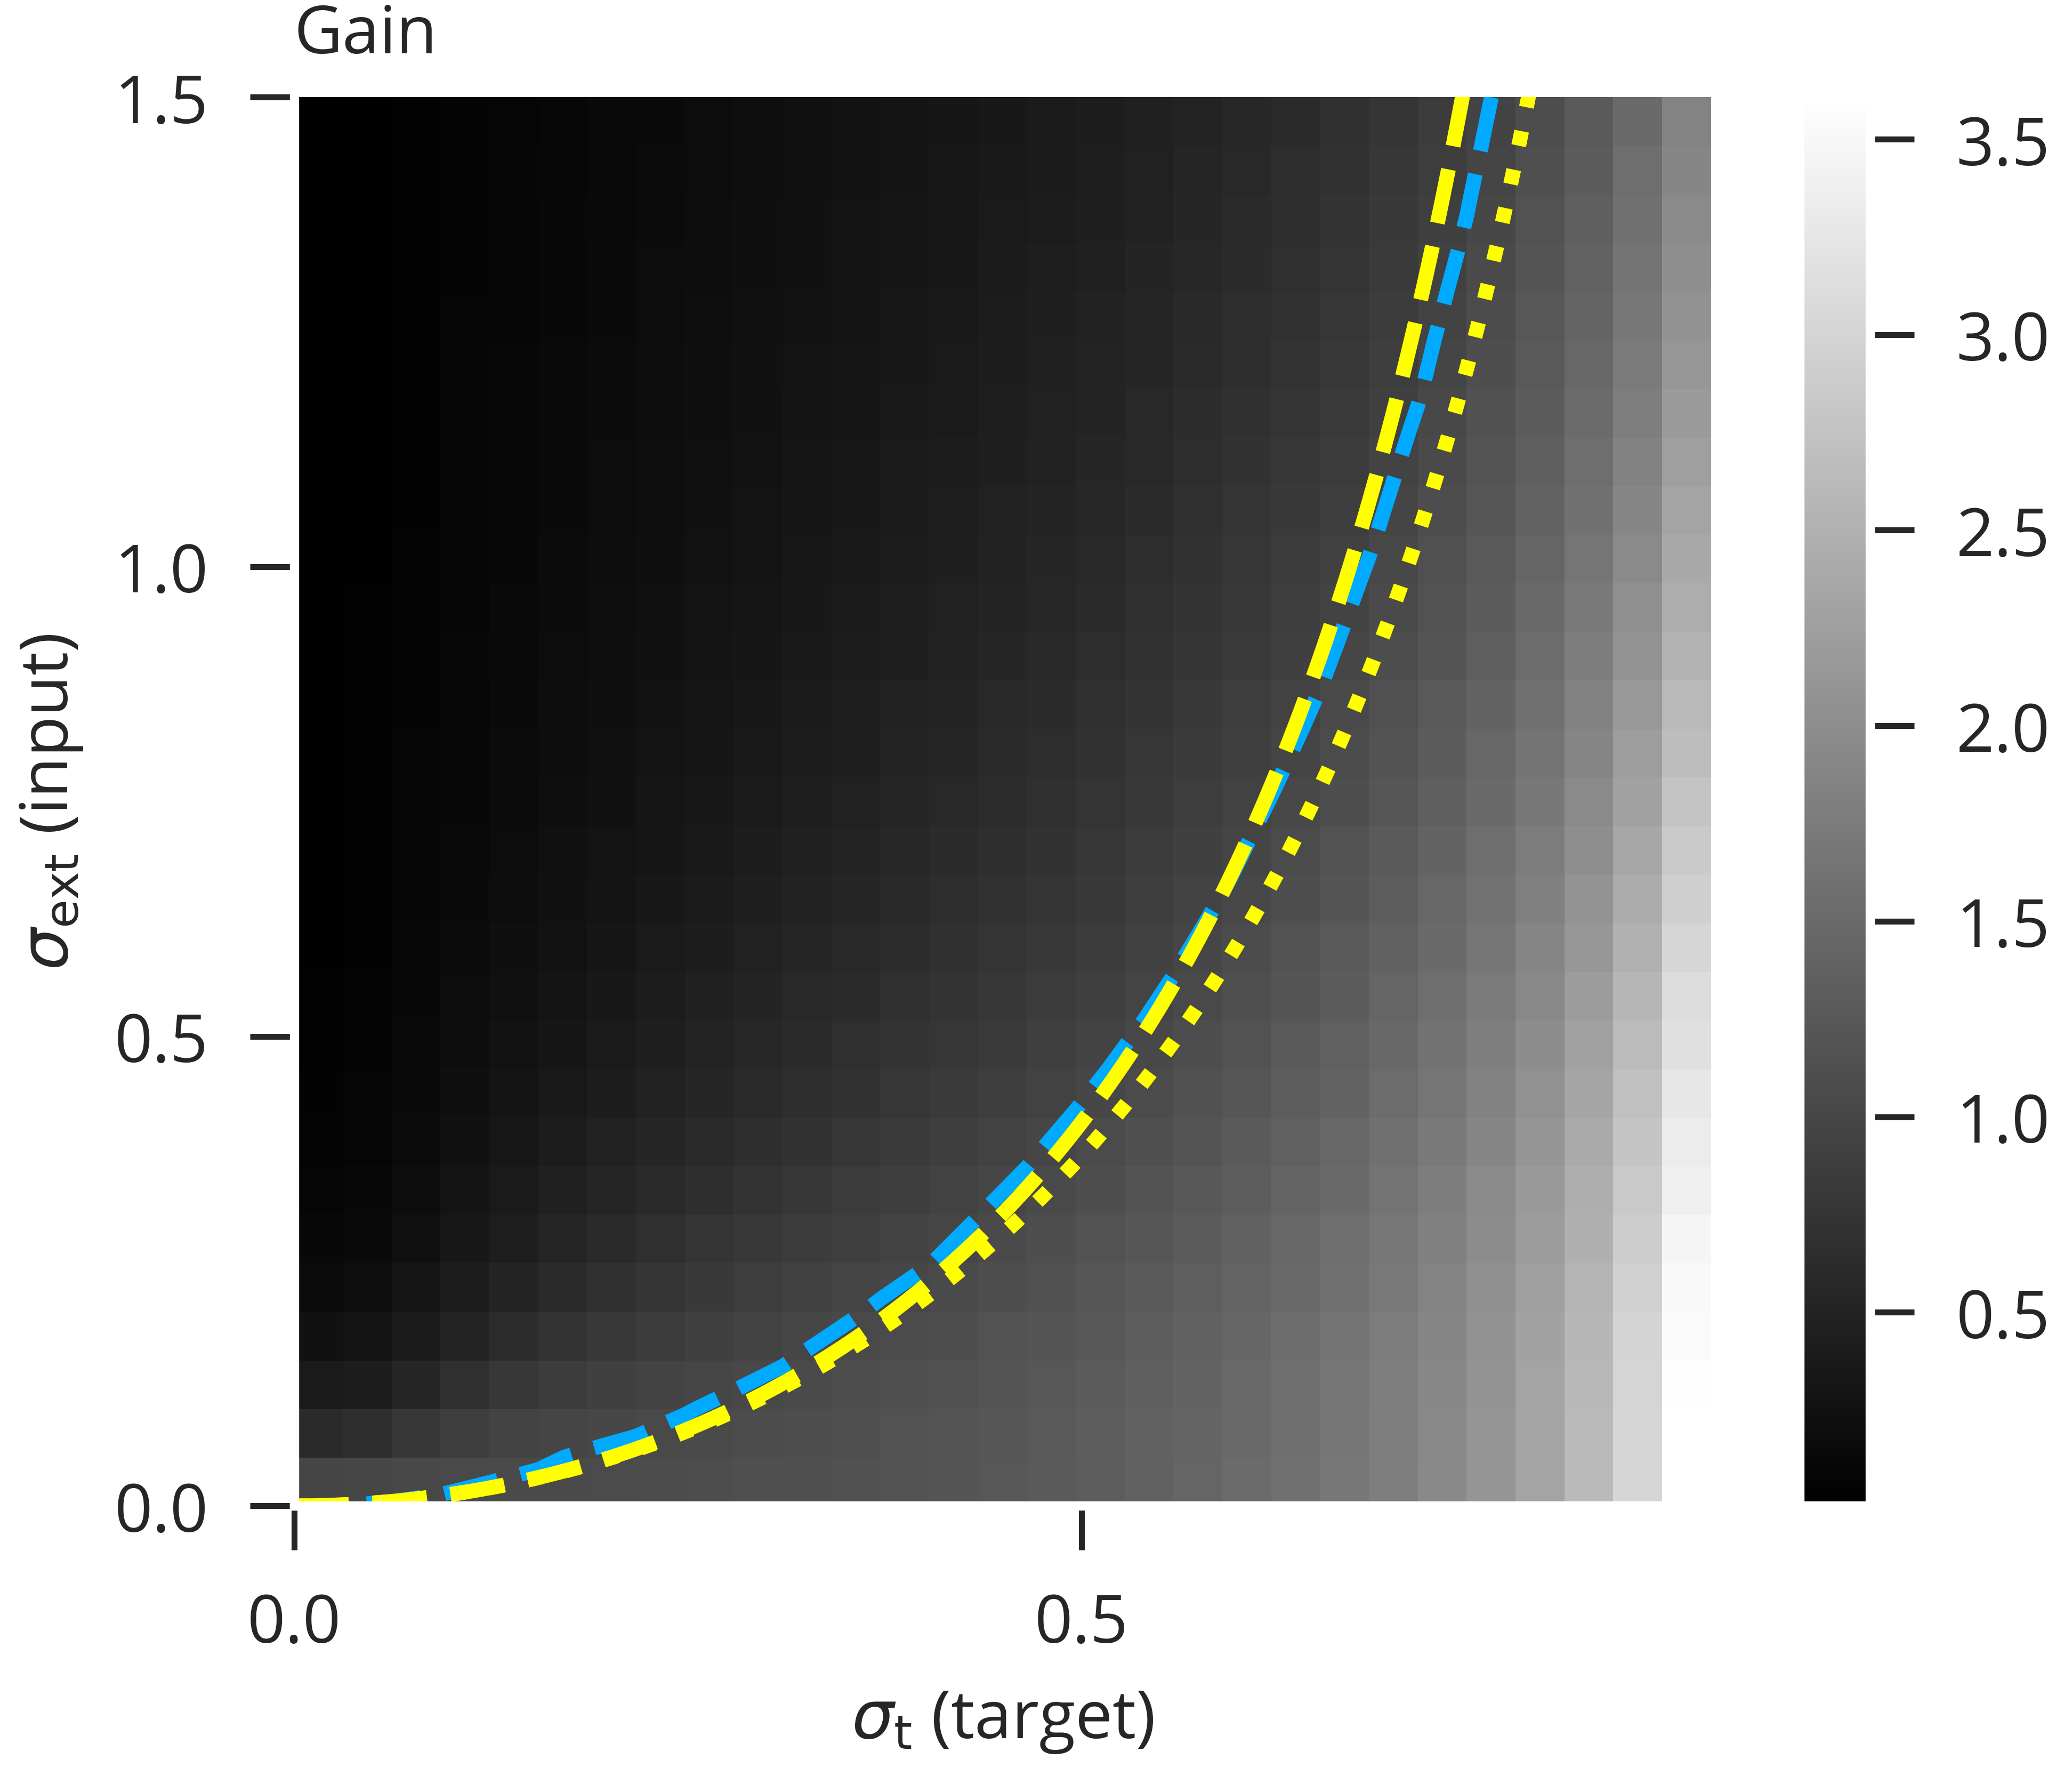
\includegraphics{./plots/theory_simulation_2.png}
	\end{center}
	\caption{{\bf Spectral Radius Transition Approximation} Blue dashed lines denotes $\langle a_i^2\rangle_{\rm P}\!=\!1/\sigma^2_{\rm w}$. Yellow dashed line is given by \eqref{eq:gauss_approx_approx}, dotted line by \eqref{eq:crit_transition_gaussian_approx}.}
	\label{Fig:theory_simulation_2}
\end{figure}

\newpage
\section{XOR-Memory Recall}	
To test the whether our self-consistent analytical approach would correctly identify the critical transition under some task-related input, we rand a sweep search over a range of values for $\sigma_{\rm ext}$ and $\sigma_{\rm t}$, using a binary sequence as input. After the initial adaptation, the network's performance  was tested with an XOR-recall task defined by
\begin{align}
f(t) &= \mathrm{XOR}\left[u(t-\tau),u(t-\tau-1)\right] \\
\mathrm{XOR}\left[x,y\right] &\defeq \begin{cases}
0 & x=y\\
1 & \text{else}
\end{cases}
\end{align}
where $u(t) \in \{-1,1\}$. The performance was quantified by the total XOR memory capacity given by
\begin{align}
\mathrm{MC}_{\rm XOR} &\defeq \sum_{k=1}^\infty \mathrm{MC}_{{\rm XOR},k} \label{eq:MC_XOR}\\
\mathrm{MC}_{{\rm XOR},k} &\defeq \max\limits_{w_{\rm out}} \frac{\mathrm{Cov}^2\left[\mathrm{XOR}\left[u(t-k),u(t-k-1)\right],y_{\rm out}(t)\right]_t}{\mathrm{Var}\left[\mathrm{XOR}\left[u(t),u(t-1)\right]\right]_t \mathrm{Var}\left[y_{\rm out}(t)\right]_t} \; .\label{eq:MC_XOR_k}
\end{align}
Fig.~\ref{fig:xor_task} depicts the performance results for this setup. Two different schemes were tested: The first one used independent Gaussian noise for the external input of each node during adaptation, where the standard deviation of the distribution was homogeneous across the population. For the actual performance measurement, a binary input sequence was fed into the network, using Gaussian distributed input weights that resulted in an average $\sigma_{\rm ext}$ of the same magnitude as was used during adaptation. In the second case, the same type of binary input was also used during adaptation. While the first approach yielded a good match between the expected shape of the critical transition line and the numerical result, optimal performance under a given external driving did not closely follow this transition. The second case (using only binary input) did exhibit a better correspondence between optimal performance and the critical transition. However, our theoretical predictions did not match this transition anymore.


\begin{figure}
	%\centering
	\begin{minipage}[t]{0.5\textwidth}
		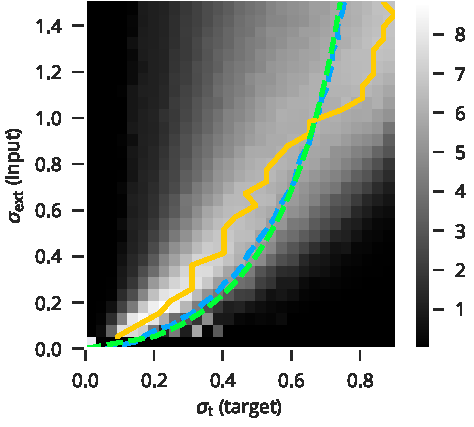
\includegraphics[width=\textwidth]{./plots/homogeneous_independent_gaussian_input_xor_perf.pdf}
	\end{minipage}
	\begin{minipage}[t]{0.5\textwidth}
		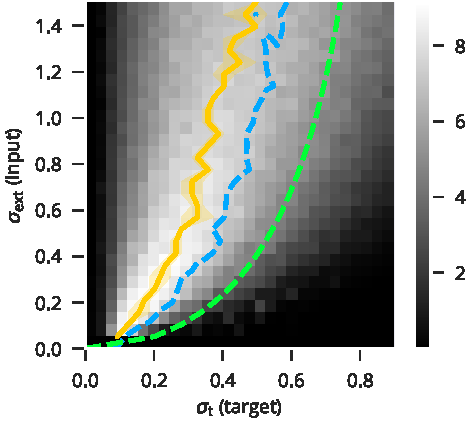
\includegraphics[width=\textwidth]{./plots/heterogeneous_identical_binary_input_xor_perf.pdf}
	\end{minipage}
	\caption{XOR-memory performance as defined in \eqref{eq:MC_XOR}. Left: Network adapted with homogeneous independent Gaussian input, tested with $\{-1,1\}$ binary input with the same standard deviation. Right: Network adapted with heterogeneous identical binary input, tested with the same input type. Blue dashed line: numerically determined points where the spectral radius is one. Orange line: maximal performance for a given $\sigma_{\rm ext}$. Green line: theoretical prediction for unit spectral radius.}
	\label{fig:xor_task}
\end{figure} 

\newpage

%	\section{Solving the Inhomogeneous Self-Consistency Equation Dynamically}\label{sec:self_consist_sol}
%	Starting with the even more general equation
%	\begin{equation}
%		\left\langle y_{{\rm y},i}^2 \right\rangle_t = \int_{-\infty}^\infty \tanh^2(x) \mathcal{N}(x,\mu_i,\sigma_i^2) \mathrm{d}x
%	\end{equation}
%	we approximated $\tanh^2(x)\approx 1-\exp(-x^2)$, which makes the integral
%	\begin{align}
%	\left\langle y_{{\rm y},i}^2 \right\rangle_t &= 1 - \frac{1}{\sqrt{2\pi \sigma_i^2}} \int_{-\infty}^\infty \exp\left(-x^2\left[1+\frac{1}{2\sigma_i^2}\right] + x\frac{\mu_i}{\sigma_i^2} - \frac{\mu_i^2}{\sigma_i^4}\right) \mathrm{d}x \\
%	&= 1-\frac{\exp\left(\frac{\mu_i^2}{4}\frac{1 + 2/\sigma_i^2}{2\sigma_i^2+1}\right)}{\sqrt{1+2\sigma_i^2}} \; . \label{eq:self_consist}
%	\end{align}
%	Under the assumption that neither recurrent weights nor node activities are correlated in time or across the population, we have
%	\begin{align}
%	\sigma^2_i &= a_i^2 N \left\langle W^2_{ij} \right\rangle_j \mathrm{Var}\left[y_j(t)\right]_{j,t} + \mathrm{Var}\left[E_i(t)\right]_t \\
%	\mu_i &= a_iN\left\langle W_{ij} \right\rangle_j\left\langle y_j(t)\right\rangle_{j,t} + \left\langle E_i(t) \right\rangle_{t} \; .
%	\end{align}
%	The condition that we would like to fulfill is $a_i^2 N \left\langle W^2_{ij}\right\rangle_j = 1 \; \forall i$. Given that we assume balanced weights $\left\langle W_{ij} \right\rangle_j = 0 \; \forall i$, this yields
%	 \begin{align}
%	 \sigma^2_i &= \mathrm{Var}\left[y_j(t)\right]_{j,t} + \mathrm{Var}\left[E_i(t)\right]_t \\
%	 \mu_i &= \left\langle E_i(t) \right\rangle_{t} \; .
%	 \end{align}
%	 If the mean of the input was zero, \eqref{eq:self_consist} would become the previously state condition
%	 \begin{equation}
%	 	\left\langle y^2_i \right\rangle_t = 1-1/\sqrt{1+2\mathrm{Var}\left[y_j(t)\right]_{j,t} + 2 \mathrm{Var}\left[E_i(t)\right]_t} \; .
%	 \end{equation}
%	 We are facing the problem that this does not have a general analytical solution. However, we can try to dynamcially solve this equation by simply measuring the right hand side of the equation during adaptation and setting this as a target value for $\left\langle y^2_i \right\rangle_t$. We implemented this using the following update rules (on top of the usual network dynamics):
%	 \begin{align}
%	 \mu_{{\rm y},i}(t) &= (1-\epsilon_\mu)\mu_{{\rm y},i}(t-1) + \epsilon_\mu y_i(t) \\
%	 \mu_{{\rm e},i}(t) &= (1-\epsilon_\mu)\mu_{{\rm e},i}(t-1) + \epsilon_\mu X_{{\rm e},i}(t) \\
%	 \sigma^2_{{\rm y},i}(t) &= (1-\epsilon_\sigma)\sigma^2_{{\rm y},i}(t-1) + \epsilon_\sigma \left[y_i(t) - \mu_{{\rm y},i}(t)\right]^2 \\
%	 \sigma^2_{{\rm e},i}(t) &= (1-\epsilon_\sigma)\sigma^2_{{\rm e},i}(t-1) + \epsilon_\sigma \left[X_{{\rm e},i}(t) - \mu_{{\rm e},i}(t)\right]^2 \\
%	 y^2_{{\rm targ},i}(t) &= 1 - 1/\sqrt{1+2\left\langle\sigma^2_{{\rm e},j}(t)\right\rangle_j + 2\sigma^2_{{\rm e},i}(t) } \\
%	 a_i(t) &= a_i(t-1) + \epsilon_{\rm a} \left(y^2_{{\rm targ},i}(t) - y^2_i(t)\right) \\
%	 b_i(t) &= b_i(t-1) + \epsilon_{\rm b} y_i(t)
%	 \end{align}
%	 As shown in Fig.~\ref{fig:gain_dyn_self_consist}, this mechanism is actually quite bad at tuning gains to appropriate values (the quantity shown in the plot should converge to one). Interestingly, the resulting spectral radius after adaptation is not as far off the target of unit radius as the individual gains suggest, see Fig.~\ref{fig:eigvals_self_consist}. Still we see quite a lot of bunching at the origin, which is caused by heterogeneity in $a_i^2 N \left\langle W^2_{ij}\right\rangle_j$ as shown in the first plot. One reason for this is the fact that the approximation for the variance of the recurrent input is very far from accurate, as seen in Fig.~\ref{fig:recurr_var_predict_self_consist}. Since this is a crucial part of our approach to setting our target variance, we cannot expect to get good results.
%	 \begin{figure}
%	 	\centering
%	 	\includegraphics{./plots/gain_dyn_self_consist.pdf}
%	 	\caption{Gain dynamics as described in section \ref{sec:self_consist_sol}.}
%	 	\label{fig:gain_dyn_self_consist}
%	 \end{figure}
% 
%	 \begin{figure}
%	 	\centering
%	 	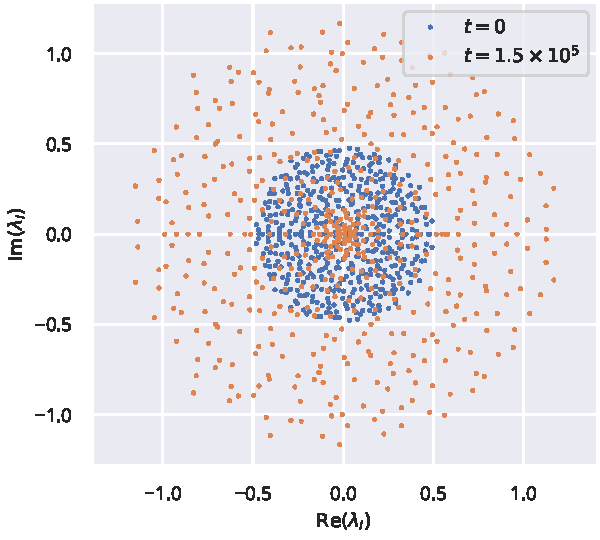
\includegraphics{./plots/eigvals_self_consist.pdf}
%	 	\caption{Effective eigenvalues before and after adaptation as described in section \ref{sec:self_consist_sol}.}
%	 	\label{fig:eigvals_self_consist}
%	 \end{figure}
% 
	 	
\section{A scaling mechanism estimating the phase space contraction rate}\label{sec:self_consist_sol_local}
As we have seen, the previous approach did not yield the desired results. However, we may take a slightly different approach to this problem by stating that the essential property that we are trying to reach is that a mapping from neural activities at time step $t-1$ to the recurrent membrane potential at $t$ should, on average, neither be contracting nor expanding. That is
\begin{equation}
\left\langle \frac{||\mathbf{X}_{\rm r}(t)||^2}{||\mathbf{y}(t-1)||^2}\right\rangle_t = 1 \; .
\end{equation}
Being aware that we do not necessarily find exact equality, we can also demand that
\begin{align}
\frac{\left\langle ||\mathbf{X}_{\rm r}(t)||^2\right\rangle_t}{\left\langle ||\mathbf{y}(t-1)||^2\right\rangle_t} &= 1 \\ \left\langle ||\mathbf{X}_{\rm r}(t)||^2\right\rangle_t &= \left\langle||\mathbf{y}(t-1)||^2\right\rangle_t \; .
\end{align}
Note that previously we already assumed to have access to a mean field over the square of neural activities. If we assume that we can also access a mean field over recurrent membrane potentials, this allows us to modify the gain update rule in the following way:
\begin{align}
X_{{\rm r},i}(t) &= a_i(t) \sum_{j=1}^N W_{ij} y_j(t-1)\\
a_i(t) &= a_i(t-1) + \epsilon_{\rm a} a_i(t-1) \left[ ||\mathbf{y}(t-1)||^2 - ||\mathbf{X}_{\rm r}(t)||^2 \right] \; . \label{eq:alt_mech_gain_2}
\end{align}
The proportionality factor $a_i(t-1)$ is optional and simply accounts for a ``stretching" of the gain vector proportional to the difference term.
Importantly, if the adaptation rate $\epsilon_{\rm a}$ is sufficiently slow, $||\mathbf{y}(t-1)||^2$ in \eqref{eq:alt_mech_gain_2} can be replaced by $||\mathbf{y}(t)||^2$:
\begin{equation}
	a_i(t) = a_i(t-1) + \epsilon_{\rm a} a_i(t-1) \left[ ||\mathbf{y}(t)||^2 - ||\mathbf{X}_{\rm r}(t)||^2 \right] \; . \label{eq:alt_mech_gain_3}
\end{equation}
Fig.~\ref{fig:gain_dyn_self_consist_local} and \ref{fig:eigvals_self_consist_local} show that in this implementation, the tuning towards unit spectral radius is almost perfect.

To better understand the dynamics of this mechanism, we approximate the average dynamics and reduce it to the case of a single scaling factor $a$ and $||\mathbf{y}(t)||^2$:
\begin{align}
	 \left\langle \Delta a \right\rangle_t &= \epsilon_{\rm a} a \left(1-a^2\sigma_{\rm w}^2 \right) ||\mathbf{y}(t)||^2 \label{eq:gain_dyn_approx}\\
	 \left\langle \Delta ||\mathbf{y}||^2 \right\rangle &\approx N\left[1 - \avg{\frac{1}{1+2a^2\sigma_{\rm w}^2 ||\mathbf{y}||^2 / N + 2 \sigma_{{\rm ext},i}}}{P} \right] - ||\mathbf{y}||^2 \label{eq:y_squ_dyn_approx}
\end{align}

These dynamics are depicted in Fig.~\ref{fig:gain_reg_dynsys}. One stable fixed point corresponds to the desired property for the spectral radius.

\begin{figure}
	\centering
	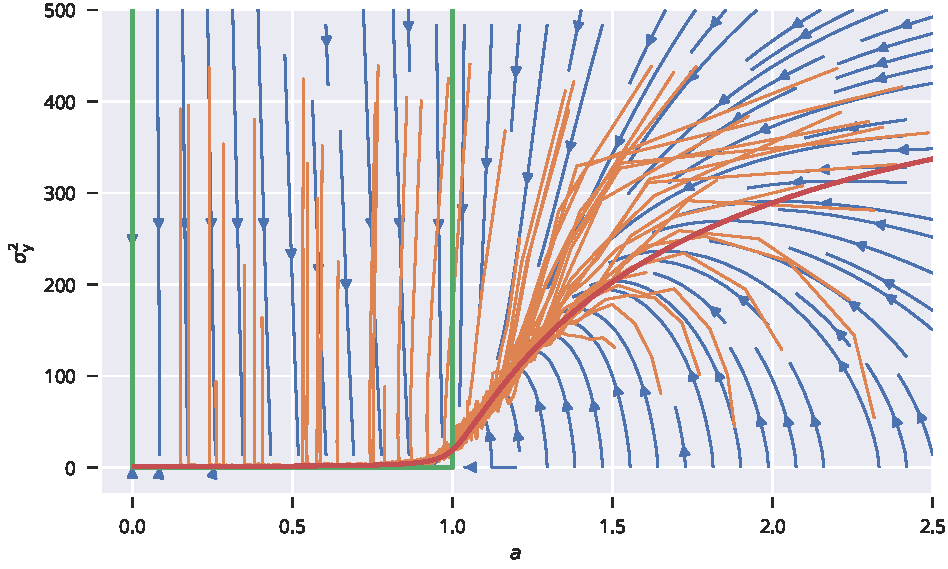
\includegraphics{./plots/heterogeneous_identical_binary_input_alt_hom_regulation.pdf}
	\caption{Dynamics of gain and squared activity as described in \eqref{eq:gain_dyn_approx} and \eqref{eq:y_squ_dyn_approx}. Shown is the flux given by the equations (blue), as well as traces of actual network/gain dynamics (orange), where the latter is given by \eqref{eq:alt_mech_gain_3}. Green and red lines depict nullclines of gain and squared activity, respectively. Input to the network was heterogeneous identical binary input. $\sigma_{\rm ext} = 0.05$, $\epsilon_{\rm a} = 0.1$.}
	\label{fig:gain_reg_dynsys}
\end{figure}

\begin{figure}
	\centering
	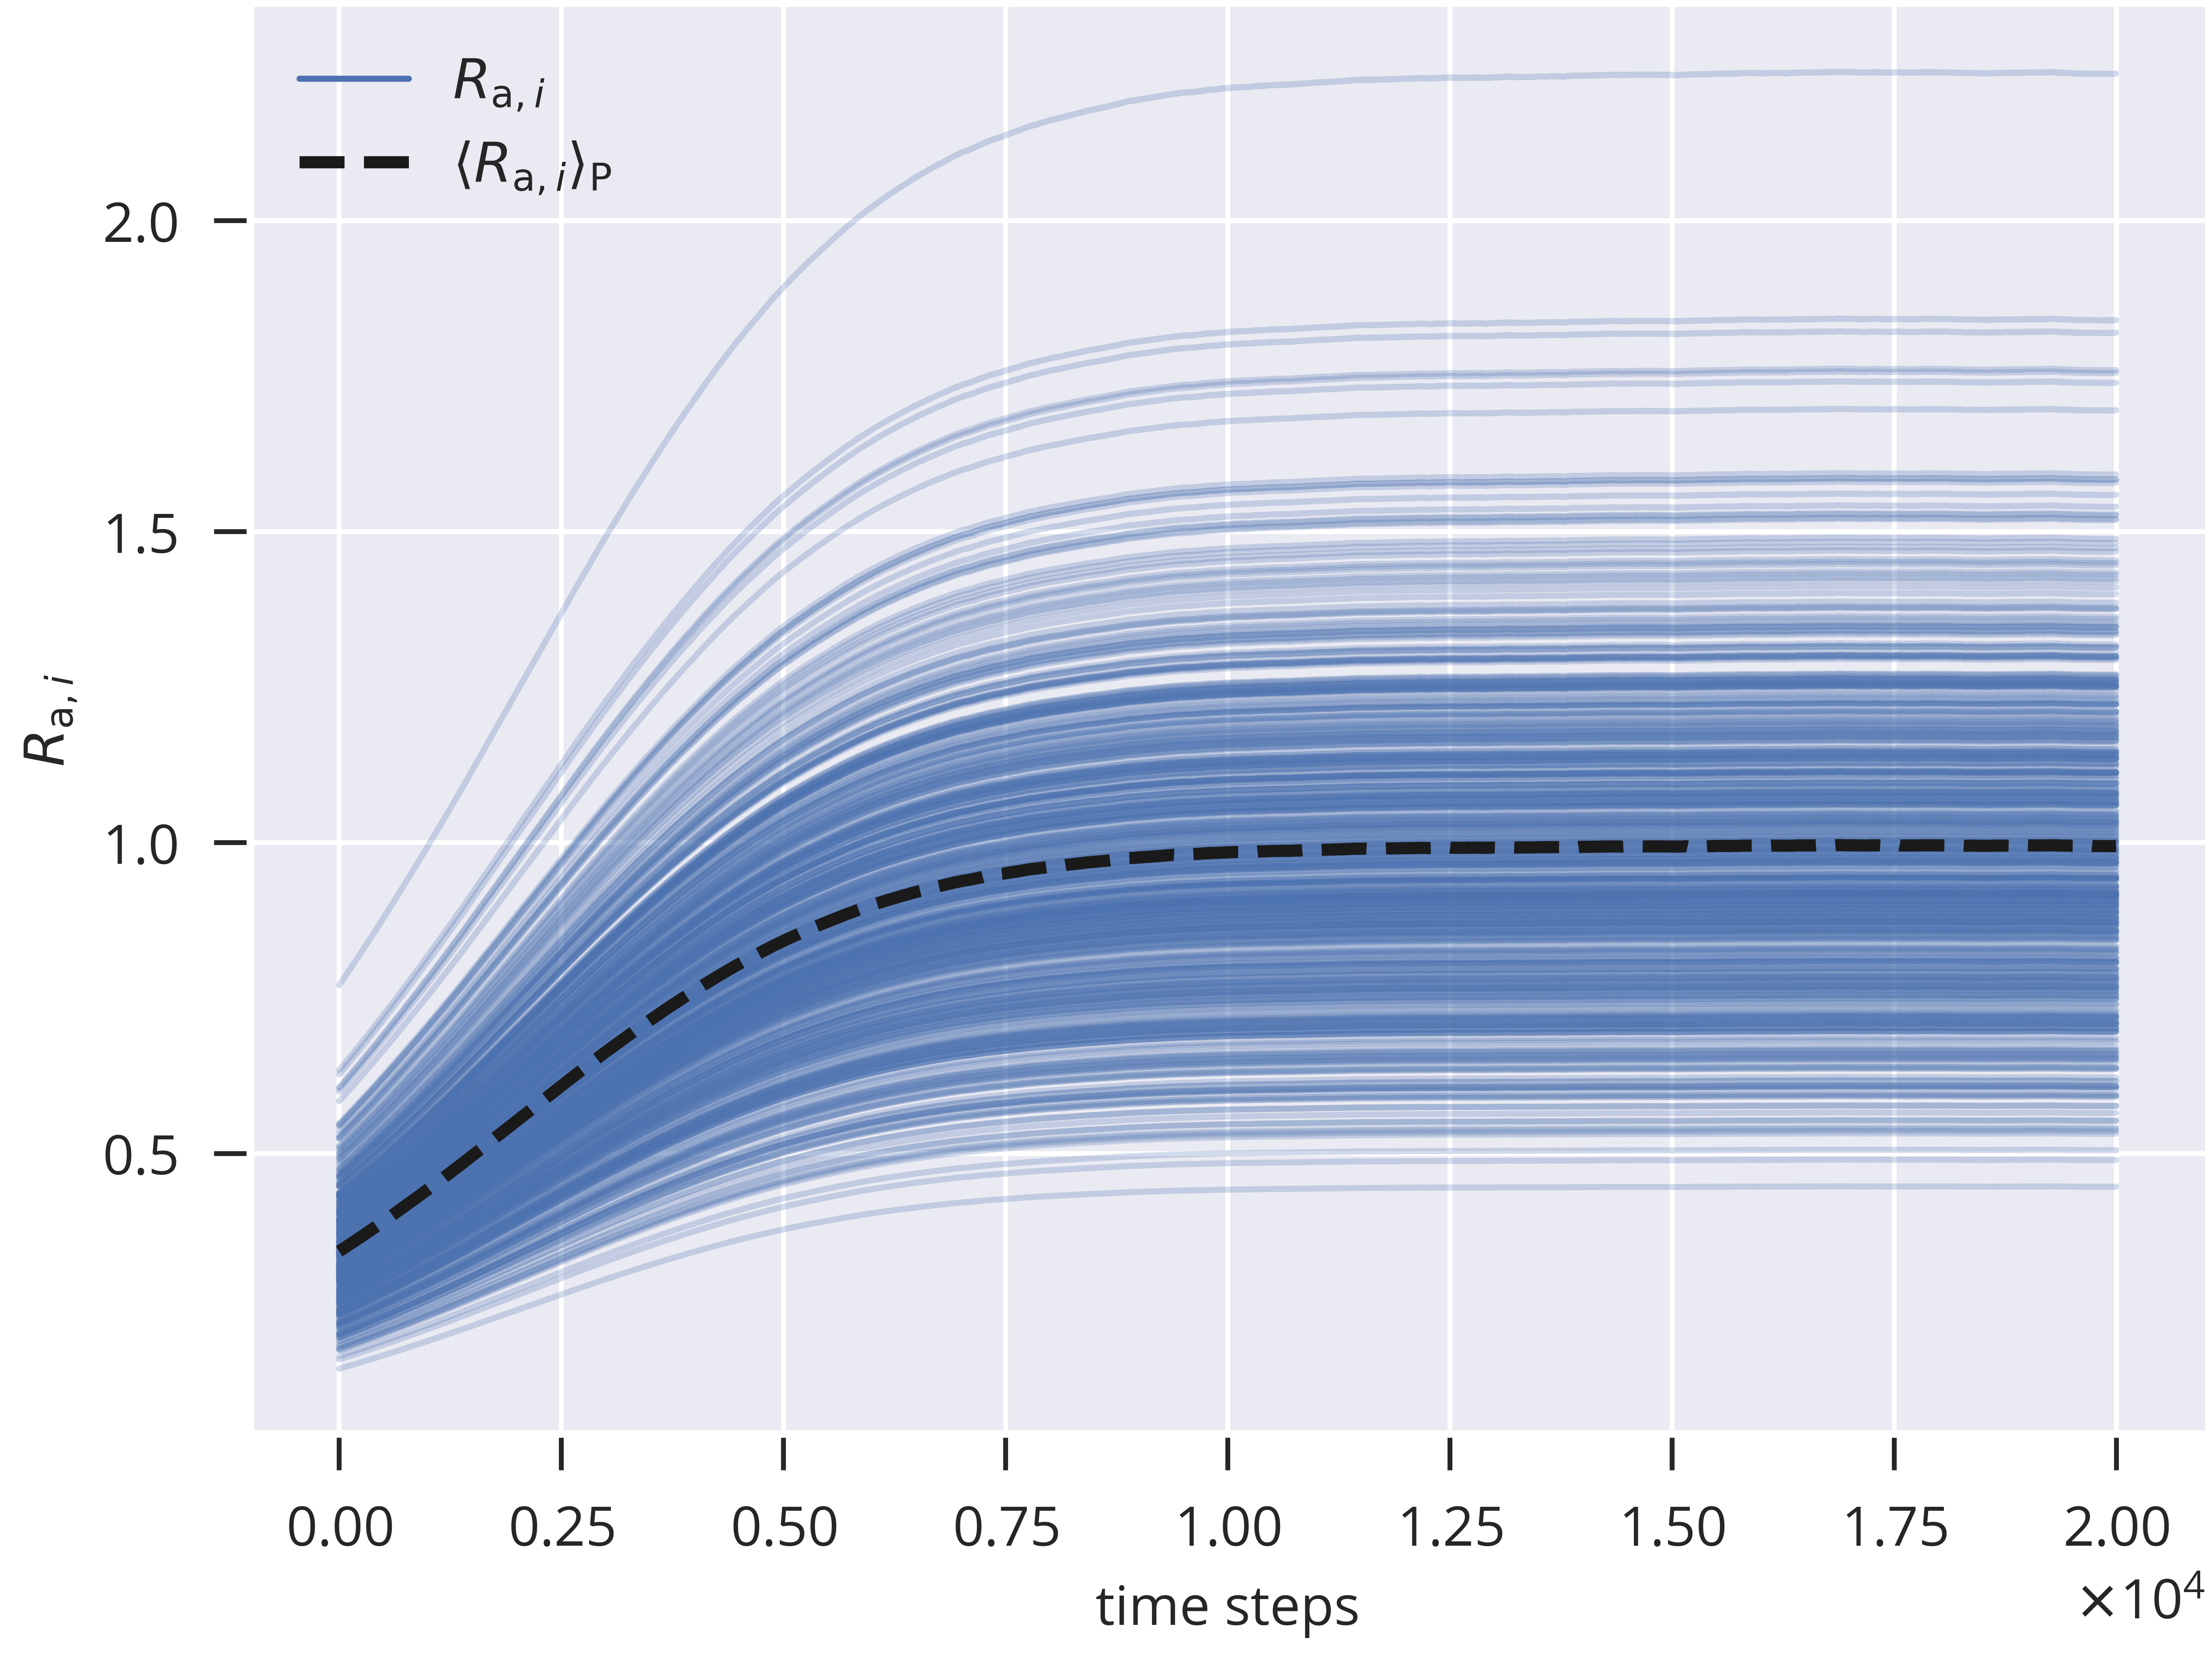
\includegraphics{./plots/heterogeneous_identical_binary_input_alt_hom_regulation_r_a.png}
	\caption{Gain dynamics as described in section \ref{sec:self_consist_sol_local},using heterogeneous identical binary input.}
	\label{fig:gain_dyn_self_consist_local}
\end{figure}

\begin{figure}
	\centering
	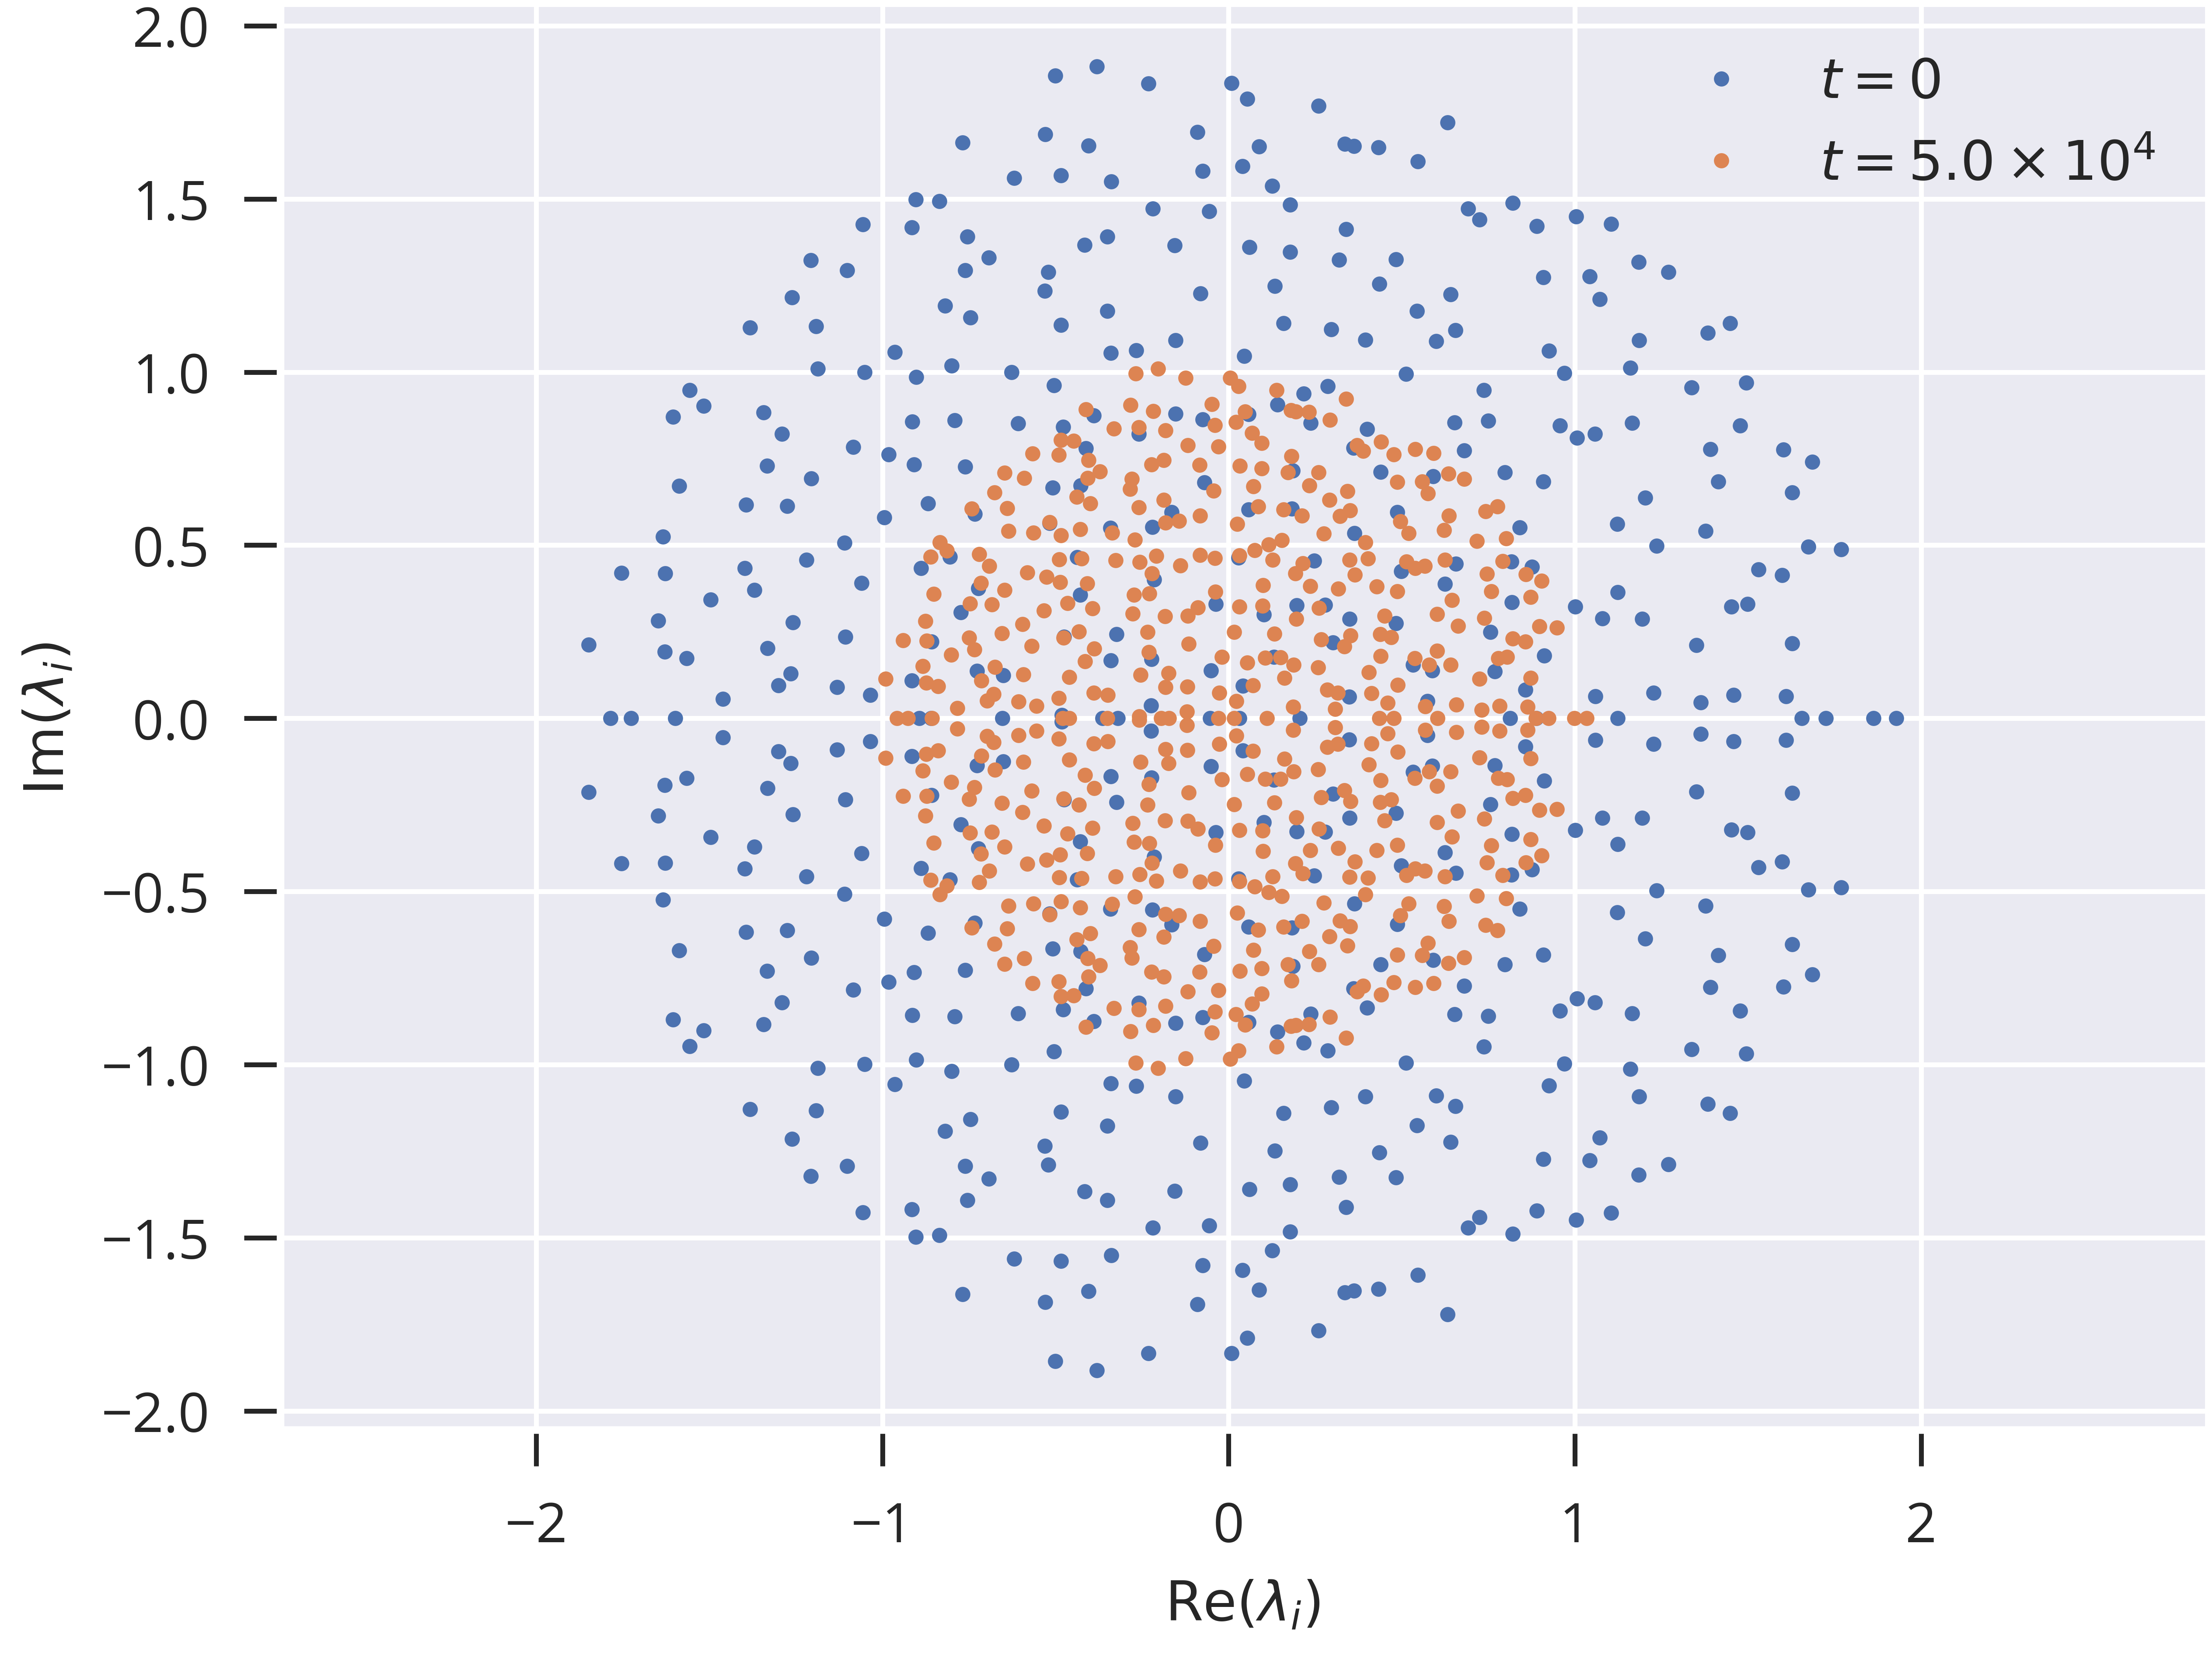
\includegraphics{./plots/heterogeneous_identical_binary_input_alt_hom_regulation_specrad.png}
	\caption{Effective eigenvalues before and after adaptation as described in section \ref{sec:self_consist_sol_local}, using heterogeneous identical binary input.}
	\label{fig:eigvals_self_consist_local}
\end{figure}	


\newpage

\begin{appendix}
			



\end{appendix}


%----------------------------------------
\section*{Conclusion}
%----------------------------------------
We have illustrated the basic format to the manuscript that you consider to
submit to Neural Computation. We hope this is helpful to the authors.

%----------------------------------------
\subsection*{Acknowledgments}
%----------------------------------------
The people you want to acknowledge. For this document, we appreciate J�rg
L�cke, author of an accepted paper who generously allowed us to use his
template.

\section*{Appendix}
\section{Gradient-Based Error-Driven Adaptation}
Instead of trying to find some heuristics that would tune the network into a state that is supposed to be ``generally suitable" for time dependent problems / series prediction, we could adapt our parameters based on an error signal. Suppose we have an error between an output signal $u(t)$ and a target signal $f(t)$, we can define the error measure
\begin{align}
\epsilon(t) &= u(t) - f(t) \\
E(t) &= \frac{1}{2}\epsilon(t)^2 \\
\mathcal{L} &= \avg{E(t)}{t}\; .	
\end{align}
A gradient-based approach to reducing $E$ with respect to $a_i$ would read
\begin{equation}
\Delta a_i \propto - \fullderiv{}{a_i} \mathcal{L} = -\avg{\fullderiv{}{a_i}E(t)}{t}
\end{equation}
One way to evaluate this expression is called \textit{backpropagation through time} (BPTT). Essentially, BPTT unfolds the gradient into the following sum:
\begin{equation}
\fullderiv{}{a_i} \mathcal{L} =  \sum_{t=-\infty}^\infty \fullderiv{\mathcal{L}}{\mathbf{y}(t)}\partderiv{\mathbf{y}(t)}{a_i} \label{eq:BPTT}
\end{equation}
Partial derivatives with respect to neural activities are calculated for each time step and the full derivatives of the error with respect to these activities can be subsequently calculated via the chain rule, going ``backwards" in time. This method does requires the evaluation of $\fullderiv{\mathcal{L}}{\mathbf{y}(t)}$ to be truncated at some point, obviously. An alternative, known as \textit{real time recurrent learning} (RTRL) calculates full derivatives of activities with respect to the parameter, but only partial derivatives of the error measure with respect to these activities:
\begin{align}
\fullderiv{}{a_i} \mathcal{L} = \sum_{t=-\infty}^\infty \partderiv{\mathcal{L}}{\mathbf{y}(t)}\fullderiv{\mathbf{y}(t)}{a_i} \label{eq:RTRL}
\end{align}
the product between the two vectors has to be interpreted as a scalar product. Mathematically, these expressions are exactly equivalent, but in practice, lead to different implementations. We can see this more clearly by plugging in the definition of the error measure.

BPTT:
\begin{align}
\fullderiv{}{a_i} \mathcal{L} &=  \sum_{t=-\infty}^\infty \fullderiv{\avg{E(t')}{t'}}{\mathbf{y}(t)}\partderiv{\mathbf{y}(t)}{a_i} \\
&= \lim_{T\to\infty} \frac{1}{2T+1} \sum_{t'=-T}^T \sum_{t=-\infty}^\infty \fullderiv{E(t')}{\mathbf{y}(t)} \partderiv{\mathbf{y}(t)}{a_i} \\
\end{align}
Since our model does not contain causation backwards in time, we can cut the sum by
\begin{equation}
\fullderiv{}{a_i} \mathcal{L} = \lim_{T\to\infty} \frac{1}{2T+1} \sum_{t'=-T}^T \sum_{t=-\infty}^{t'} \fullderiv{E(t')}{\mathbf{y}(t)} \partderiv{\mathbf{y}(t)}{a_i}
\end{equation}
In the case of stochastic gradient descent, this is split up into a series of $\Delta a_i(t)$ that is subsequently added to the parameter where
\begin{equation}
\Delta a_i(t') = - \epsilon_a \sum_{t=-\infty}^{t'} \fullderiv{E(t')}{\mathbf{y}(t)} \partderiv{\mathbf{y}(t)}{a_i} \; .
\end{equation}
Furthermore, as mentioned before, this sum has to be truncated at some point:
\begin{equation}
\Delta a_i(t') \approx - \epsilon_a \sum_{t=t' - t_{\rm trunc}}^{t'} \fullderiv{E(t')}{\mathbf{y}(t)} \partderiv{\mathbf{y}(t)}{a_i} \; . \label{eq:stoch_grad_BPTT}
\end{equation}

Proceeding in the same way with \eqref{eq:RTRL}, we get
\begin{equation}
\fullderiv{}{a_i} \mathcal{L} = \lim_{T\to\infty} \frac{1}{2T+1} \sum_{t'=-T}^T \sum_{t=-\infty}^\infty \partderiv{E(t')}{\mathbf{y}(t)} \fullderiv{\mathbf{y}(t)}{a_i} \\
\end{equation}
Similar to the causal argument in BPTT, we find that $\partderiv{E(t')}{\mathbf{y}(t)}$ is only nonzero if $t=t'$, which allows us to drop the inner sum entirely:
\begin{equation}
\fullderiv{}{a_i} \mathcal{L} = \lim_{T\to\infty} \frac{1}{2T+1} \sum_{t=-T}^T  \partderiv{E(t)}{\mathbf{y}(t)} \fullderiv{\mathbf{y}(t)}{a_i} \\
\end{equation}
Again, stochastic gradient descent splits up this sum into subsequent changes:
\begin{equation}
\Delta a_i(t) = -  \epsilon_a \partderiv{E(t)}{\mathbf{y}(t)}\fullderiv{\mathbf{y}(t)}{a_i}
\end{equation}
While this might seem like a simpler expression than \eqref{eq:stoch_grad_BPTT}, the challenge of this approach is to evaluate the \emph{full} derivative $\fullderiv{\mathbf{y}(t)}{a_i}$ in each time step. Practically, this is done in an iterative way:
\begin{equation}
\fullderiv{\mathbf{y}(t)}{a_i} = \partderiv{\mathbf{y}(t)}{a_i} + \left[\partderiv{\mathbf{y}(t)}{\mathbf{y}(t-1)}\right] \fullderiv{\mathbf{y}(t-1)}{a_i} \; . \label{eq:RTRL_deriv_it}
\end{equation}
Note that the expression $\partderiv{\mathbf{y}(t)}{\mathbf{y}(t-1)}$ is a rank two tensor where $\left[\partderiv{\mathbf{y}(t)}{\mathbf{y}(t-1)}\right]_{ij} = \partderiv{y_i(t)}{y_j(t-1)}$. A problem with this iterative approach is that, if used in combination with stochastic gradient descent, $a_i$ will change while iteratively updating the derivatives. This means that derivatives are only exact in the ``adiabatic" limit of very small learning rates.

\subsection{Biological Plausibility in Backpropagation}

The question how a backpropagation scheme could be implemented in the brain is an ongoing research field (see e.g. \cite{Whittington_2019}). A particular variant of this question is how causal relations over time in a recurrent network could be learned in a biologically plausible fashion. Comparing the previously discussed frameworks, it appears to be the case that RTRL is a better candidate for this question: In each instance time instance, the update rule only consists of two terms that can be interpreted rather easily: A term that accounts for the effect of neural activities on the error signal, and a term that expresses the effects of changes in the actual parameters onto these activities. Some recent approaches to biologically plausible learning (see \cite{Murray_2019,Bellec_2019}) have essentially proposed to drop the second iterative term in \eqref{eq:RTRL_deriv_it} to avoid the non-local nature of this equation. Written out in complete form, this yields
\begin{equation}
\Delta a_i(t) = -\epsilon_a \epsilon(t) W^0_i [1-y_i^2(t)] \sum_j W_{ij} y_j(t-1) \; . \label{eq:RTRL_approx}
\end{equation}
We compared this approximate learning rule for the XOR-recall task with the full RTRL rule by stochastically estimating the gradients. In Fig.~\ref{fig:RTRL_gain_dyn} we reduced the dynamics to a global gain parameter (by taking the mean over individual gain gradients) for illustration purposes and also included the actual error landscape from which the gradient was to be derived.

\begin{figure}
	\centering
	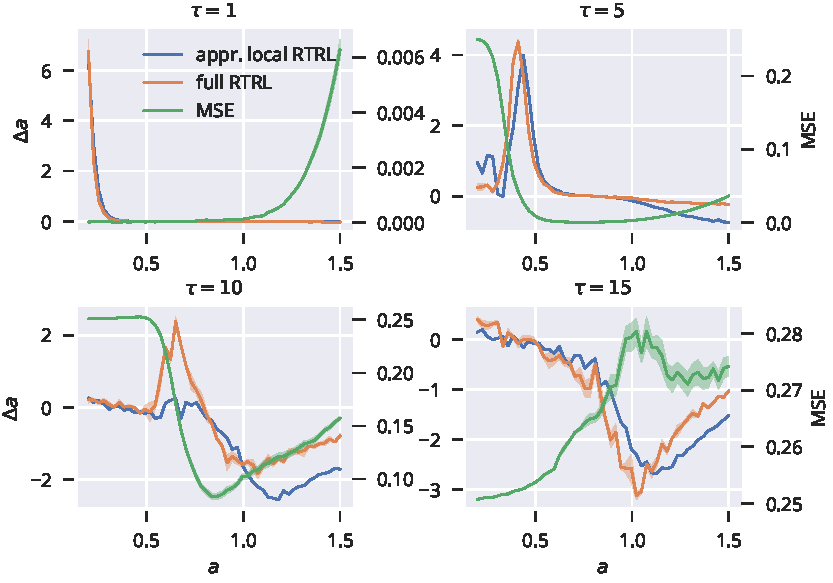
\includegraphics{./plots/delta_a_local.pdf}
	\caption{Error gradients calculated from full RTRL and from the approximation given in \eqref{eq:RTRL_approx}. Mean square error (MSE) is shown in green.}
	\label{fig:RTRL_gain_dyn}
\end{figure}

The approximate gradients are following quite closely. However, we can see that if the recall length becomes longer, an additional minimum at zero gain occurs that the gradient based adaptation could potentially end up in.

We further investigated the effect of the network size onto the shape of the objective function, see Fig.~\ref{fig:performance_network_size}. As expected, performance generally increased (MSE decreased) monotonically with increasing network size. Furthermore, larger networks can increase the width of the optimal parameter range, as seen for $\tau=5$. Another visible effect of decreasing network size is the disappearance of local minima, eventually leading to the aforementioned global minimum at zero gain. It appears that this ``catastrophic shutdown" of gains in case no good solution can be found is less of an issue for large networks. Still, since it is the optimal solution if the network can not succeed in extracting actual information from external driving (i.e., ``it is better to say nothing than to have a random guess"), it seems likely that if an actual biological system was subject to error driven adaptation, it would also use some form of homeostatic regulation to avoid this effect.

\begin{figure}
	\centering
	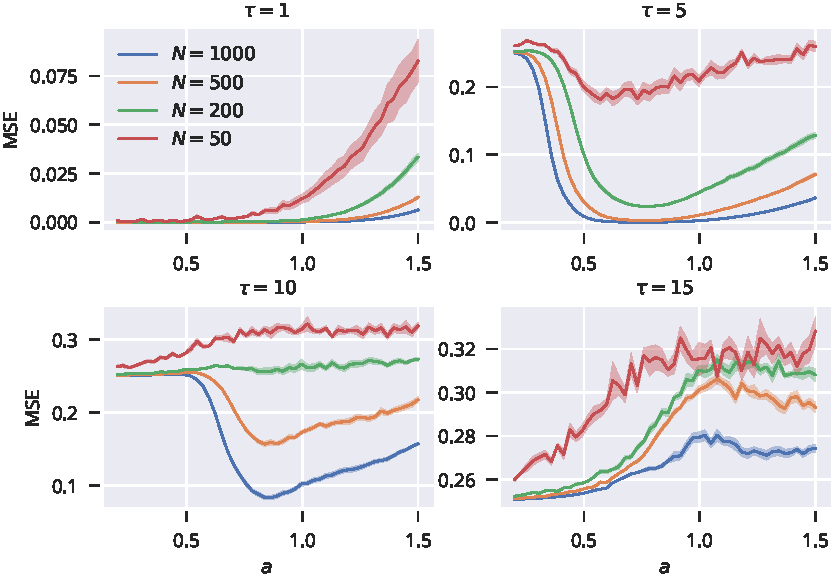
\includegraphics{./plots/performance_network_size.pdf}
	\caption{Mean square error for the XOR-recall task as a function of gain for different network sizes.}
	\label{fig:performance_network_size}
\end{figure} 

\section{Additional Figures}


\begin{figure}
	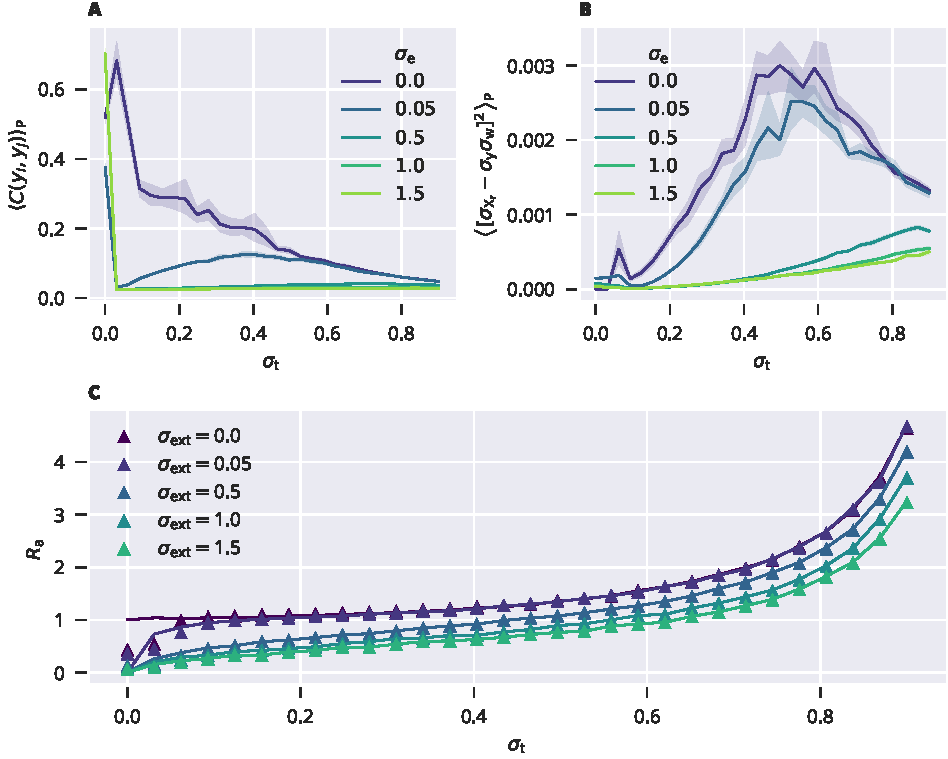
\includegraphics{./plots/heterogeneous_independent_gaussian_input_compos.pdf}
	\caption{Heterogeneous Independent Gaussian Input. {\bf A}: Population average of inter-neuron cross correlation. {\bf B}: Prediction error of recurrent input variance. {\bf C}: Theoretical prediction of $R_{\rm a}$ vs. numerical results.}
	\label{fig:gains_self_consist_het_gauss}
\end{figure}

\begin{figure}
	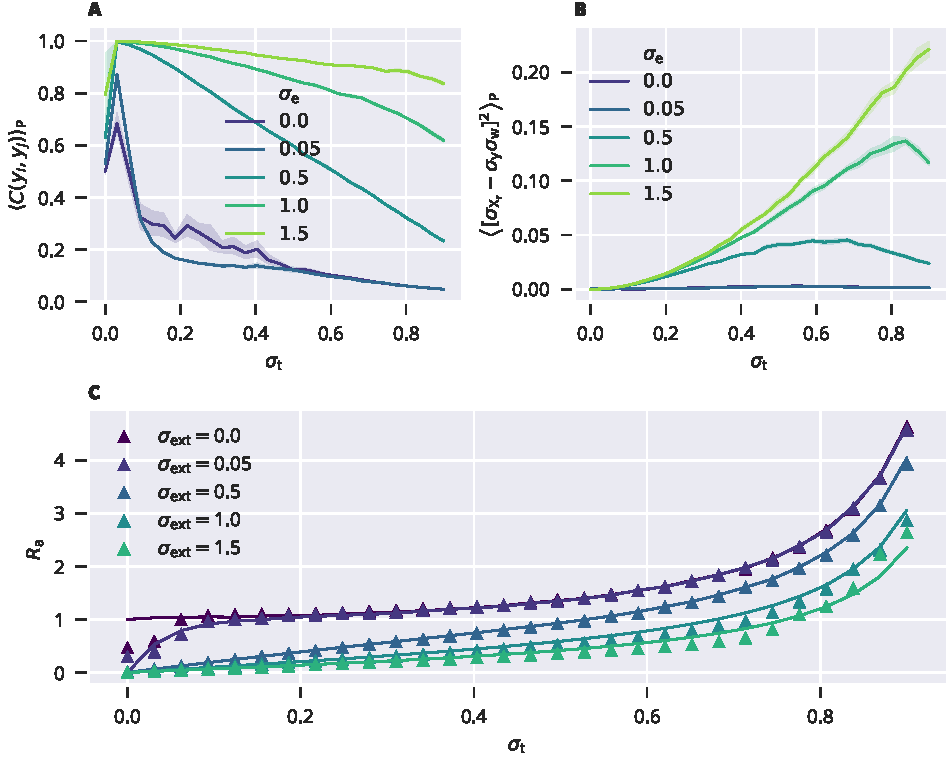
\includegraphics{./plots/homogeneous_identical_binary_input_compos.pdf}
	\caption{Homogeneous Identical Binary Input. {\bf A}: Population average of inter-neuron cross correlation. {\bf B}: Prediction error of recurrent input variance. {\bf C}: Theoretical prediction of $R_{\rm a}$ vs. numerical results.}
	\label{fig:gains_self_consist_hom_bin}
\end{figure}

\begin{figure}
	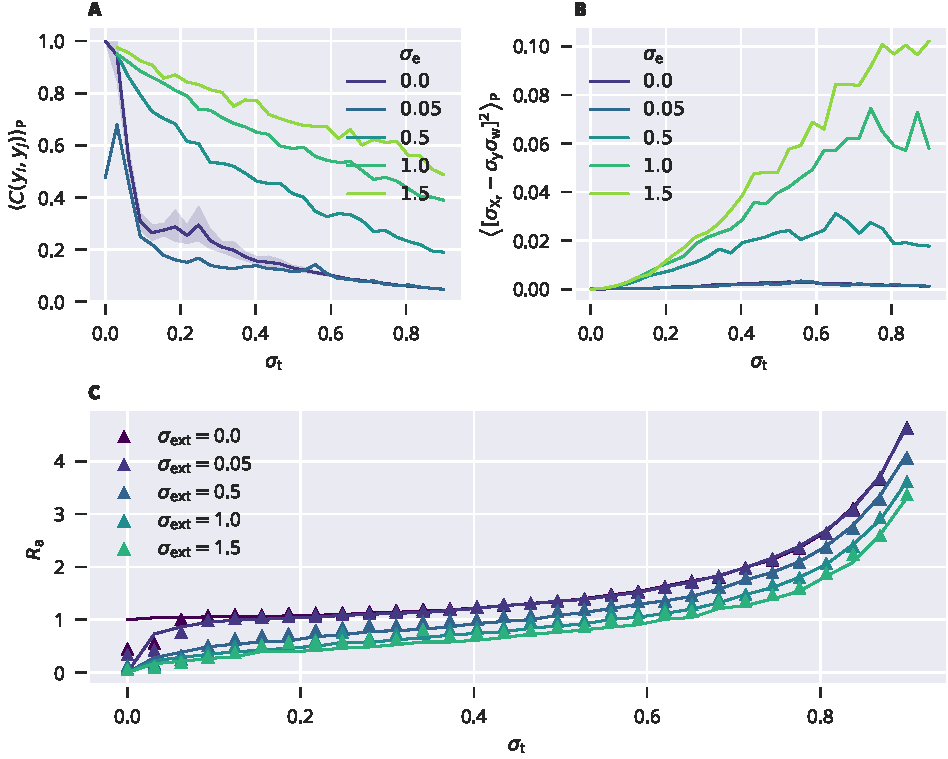
\includegraphics{./plots/heterogeneous_identical_binary_input_compos.pdf}
	\caption{Heterogeneous Identical Binary Input. {\bf A}: Population average of inter-neuron cross correlation. {\bf B}: Prediction error of recurrent input variance. {\bf C}: Theoretical prediction of $R_{\rm a}$ vs. numerical results.}
	\label{fig:gains_self_consist_het_bin}
\end{figure}

\newpage
	
	%%%%%%%%%%%%%%%%%%%%%%%%%%%%%%%%%%%%%%%%%%%%%%%%%%%%%%%
	\bibliographystyle{humannat}
	\bibliography{schubert_echo}
	%%%%%%%%%%%%%%%%%%%%%%%%%%%%%%%%%%%%%%%%%%%%%%%%%%%%%%%
	
\end{document}